% =====================================================================
%  body.tex  --  section content for the KSN / Acta Astronautica paper
%  Class-agnostic: \input by both main.tex (elsarticle) and qa.tex.
% =====================================================================

\section{Introduction}
\label{sec:intro}

In a landmark 1964 paper, \citet{Kardashev1964} proposed a universal scale for
classifying the technological advancement of civilisations by their total rate of
energy consumption. A Type~I civilisation harnesses all the energy available on its
home planet --- \citet{Kardashev1964} estimated Earth's total expenditure at the time
at $4\times10^{12}$~W --- a Type~II civilisation consumes the entire energy output of
its host star ($L_\odot \approx 3.828\times10^{26}$~W), and a Type~III civilisation
commands the output of its host galaxy. Adopting a conservative growth rate of one
percent per year, \citet{Kardashev1964} calculated that humanity would reach Type~II
status in approximately $3{,}200$ years and Type~III in approximately $5{,}800$ years.

The scale's enduring scientific importance is observational: it defines the targets of
the search for extraterrestrial intelligence (SETI). The canonical realisation of a
Type~II civilisation is a Dyson sphere or swarm --- an artificial structure
intercepting a star's full luminosity \citep{Dyson1960} --- whose reprocessed waste
heat would appear as an anomalous mid-infrared excess. This prediction has driven a
sustained observational programme: the IRAS-based whole-sky upper limit on Dyson
spheres \citep{Carrigan2009}, the $\hat{G}$ infrared search for civilisations with
large energy supplies \citep{Wright2014}, and recent candidate searches combining
Gaia DR3, 2MASS, and WISE photometry \citep{Suazo2024}. To date these surveys have
yielded no confirmed Type~II technosignature. The theoretical and observational
foundations of the field are reviewed comprehensively by \citet{LingamLoeb2021} and,
most recently, in the first dedicated SETI textbook of \citet{Wright2026}.

The Kardashev scale has been extended and critiqued in several directions.
\citet{Gray2020} refined its definitions and resolved long-standing ambiguities;
\citet{Barrow1998} proposed a complementary ``inward'' scale, ranking a civilisation's
mastery of progressively smaller length scales rather than larger energy budgets. Most
relevant to the present work, \citet{Ivanov2020} argued that contemporary searches are
calibrated to detect only civilisations that share our own ``more-is-better'' energy
philosophy, and suggested that the persistent failure of Dyson-sphere searches may
reflect the inadequacy of that assumption rather than the absence of civilisations.
This paper supplies the quantitative counterpart to that qualitative argument: a
statistical falsification, against six decades of data, of precisely the unbounded
exponential growth on which the energy-scaling Type~II target rests --- together with
the observational consequence that follows from it.

Despite its influence, the Kardashev scale carries a limitation that has received
little quantitative attention. \citet{Kardashev1964}, \citet{Sagan1973}, and
\citet{ShklovskiiSagan1966} all noted that an advanced civilisation must be
characterised not only by its energy throughput but by the information richness of what
it does with that energy; \citet{Sagan1973} proposed that a civilisation's state should
reflect its capacity to secure and transmit vast quantities of information, and
suggested a binary-tree data structure as a measure of informational complexity.
Neither author, however, formalised this requirement as a quantitative variable within
the framework. A civilisation that wastes energy inefficiently is rated identically, on
the Kardashev scale, to one that channels the same power into sophisticated
computation. The Kardashev state variable --- power, in watts --- is therefore
dimensionally incomplete as a measure of civilisational advancement: it captures the
quantity of energy consumed but not the quality of its use.

A second limitation emerges from direct comparison with data. When the one-percent
exponential model of \citet{Kardashev1964} is compared against six decades of observed
total global energy production \citep{Ritchie2022} --- used here as a valid upper-limit
proxy for consumption, since production necessarily equals or exceeds consumption at the
civilisational scale and the two track each other closely over decadal baselines --- the
model diverges substantially from the data. A linear model fits the same data
exquisitely, yet when extrapolated to the Type~II threshold it predicts a transition
timescale of order $10^5$ Hubble times: a physical \emph{reductio ad absurdum}. We term
this conflict \emph{Kardashev's Conundrum}: no \emph{statistically adequate} fit to the
observed energy record --- and the data cannot distinguish the linear fit from a free-rate
exponential --- simultaneously yields a physically coherent Type~II timescale, the linear
form giving a cosmologically absurd transition time.

Two results follow. First, the Conundrum has an immediate observational payoff for
SETI. If the energy-scaling Type~II threshold is physically unreachable, then Type~II
energy-harvesting technosignatures are unlikely ever to exist or be observed. We develop
this in Section~\ref{sec:technosignatures} as a quantitative entry in
\citeauthor{Cirkovic2018}'s \citeyearpar{Cirkovic2018} ``logistic'' category of
Fermi-paradox solutions, where it joins --- and is reinforced by --- the independent
waste-heat \citep{BalbiLingam2025} and luminosity-limit \citep{HaqqMisra2025b}
constraints on sustained technological growth. Second, the Conundrum motivates a
constructive repair. To resolve it we propose the Kardashev--Sagan--Nakamoto (KSN)
model, constructed by renormalising the energy-production ordinate by the annual average
Bitcoin network hashrate $H(t)$. The resulting state variable $B = P/H$, in units of
$\mathrm{J\,Hash^{-1}}$ --- which we term the KarNak unit --- connects energy to
irreversible computational work via the Landauer limit \citep{Landauer1961} and fulfils
the information-richness requirement identified but never quantified by
\citet{Kardashev1964} and \citet{Sagan1973}. The Bitcoin hashrate is used here strictly
as a measurement proxy: it is, at present, the only publicly auditable, unforgeable, and
continuously updated global record of proof-of-work computation, and the renormalisation
introduces no free parameter beyond those of the original model.

The notion that civilisational advancement is measured by the efficiency with which
energy is converted into organised information is an ancient one. The Antikythera
mechanism, recovered from a first-century BC shipwreck, is widely recognised as the
earliest known analogue computational device \citep{Freeth2021}; built from bronze gears
of remarkable tolerance, it converted mechanical energy into astronomical information
with a sophistication not matched in Europe for over a millennium. From Babbage's
difference engine through Turing's theoretical foundations of computation
\citep{Swade2017} to the application-specific integrated circuits (ASICs) that today
secure the Bitcoin network, humanity has followed a continuous trajectory of reducing
the energy cost per unit of computational work. The KSN model is the quantitative
expression of this trajectory: the KSN variable $B(t)$ spans fourteen orders of
magnitude over 2009--2024, tracing the same energy-to-computation efficiency gradient
from the CPU era to modern ASICs.

This paper is organised as follows. Section~\ref{sec:analysis} describes the data
(Section~\ref{sec:data}) and presents the statistical core: the assessment of the
standard Kardashev model (Section~\ref{sec:standard}), the linear model and the
Conundrum (Section~\ref{sec:linear}), Bayesian model comparison via MCMC and WAIC
(Section~\ref{sec:mcmc}), the KSN renormalisation and its physical motivation
(Section~\ref{sec:ksn}), civilisational timescales on the KSN scale
(Section~\ref{sec:timescales}), and the independence-property objection to exponential
growth (Section~\ref{sec:independence}). Section~\ref{sec:discussion} opens with the
observational consequence for Type~II technosignatures
(Section~\ref{sec:technosignatures}) before turning to falsifiability
(Section~\ref{sec:falsifiability}), limitations (Section~\ref{sec:limitations}), the
novel reading of Kardashev's two growth rates (Section~\ref{sec:growthrates}), and the
connection to the Drake equation (Section~\ref{sec:drake}).
Section~\ref{sec:conclusions} presents our conclusions.

% =====================================================================
\section{The Kardashev Conundrum and the Kardashev--Sagan--Nakamoto Model}
\label{sec:analysis}

We now present our central analysis. We compare the standard Kardashev one-percent
exponential model against a linear Ordinary Least-Squares (OLS) model fitted to the
total global energy-production data, and demonstrate that both models are unsatisfactory
in complementary ways. We then propose the Kardashev--Sagan--Nakamoto (KSN)
renormalisation as the minimal resolution that is simultaneously consistent with the
data and with physical causality.

\subsection{Data}
\label{sec:data}

The energy-production data $D$ consist of the world total primary energy consumption in
terawatt-hours per year ($\mathrm{TWh\,yr^{-1}}$), drawn from the Our World in Data
(OWID) energy dataset \citep{Ritchie2022}, which integrates the Energy Institute (EI)
Statistical Review of World Energy and the US Energy Information Administration (EIA)
international energy series; see \citet{Smil2017} for a comprehensive historical analysis
of the industrial-era energy trajectory. We use $N=60$ annual data points spanning
1965--2024. The OWID dataset column \texttt{primary\_energy\_consumption} reports values
using the direct primary energy accounting method, which measures the physical energy
output of each source without applying fossil-fuel-equivalent conversion factors. This
is distinct from the substitution method historically used by the Energy Institute,
which inflates non-fossil contributions (nuclear, hydro, wind, solar) by a thermal
efficiency factor ($\sim0.38$--$0.40$) to estimate the fossil-fuel input that would have
produced the same electricity. We adopt the direct method throughout because it measures
the actual rate of energy flow through civilisation --- the physical quantity that the
Kardashev scale is defined in terms of --- and avoids an accounting convention whose
magnitude grows with the renewable-energy share. We verify in
Section~\ref{sec:limitations} that all qualitative conclusions hold under the
substitution method.

All energy values are converted to SI watts ($\mathrm{J\,s^{-1}}$) assuming uniform power
delivery over each calendar year via
\begin{equation}
\label{eq:conv}
P\,[\mathrm{W}] = E\,[\mathrm{TWh\,yr^{-1}}] \times
\frac{10^{12}\,[\mathrm{Wh\,TWh^{-1}}] \times 3600\,[\mathrm{J\,Wh^{-1}}]}
     {365.25 \times 24 \times 3600\,[\mathrm{s\,yr^{-1}}]},
\end{equation}
where the numerator converts terawatt-hours to joules ($1~\mathrm{TWh}=3.6\times10^{15}$~J)
and the denominator is the number of seconds in one Julian year. The factors of $3600$
cancel, reducing Equation~(\ref{eq:conv}) to $P = E\times10^{12}/(365.25\times24)$~W.
This yields $P(1965)=4.95$~TW, in close agreement with the \citet{Kardashev1964} baseline
of $4$~TW, and $P(2024)=20.16$~TW, consistent with the International Energy Agency's
direct-method estimate of $\sim20$~TW. We set the origin of the time coordinate at
$t_0=1964$, the year of the Kardashev conjecture \citep{Kardashev1964}, so that
$t=\mathrm{year}-1964$ throughout.

The Bitcoin network hashrate data $H(t)$ are yearly averages in $\mathrm{Hash\,s^{-1}}$
for 2009--2024. These span the full history of Bitcoin mining from the CPU era
($\sim7~\mathrm{MH\,s^{-1}}$ in 2009) through the ASIC era
($\sim6.2\times10^{20}~\mathrm{H\,s^{-1}}$ in 2024), covering 16 annual data points and
14 orders of magnitude in hashrate. For 2009--2013 (the CPU and GPU eras), no single
authoritative source of annual-average hashrate exists; we derive yearly averages from
the on-chain difficulty record using the standard relation $H = D\times2^{32}/600$,
taking the logarithmic mean of the January~1 and December~31 difficulty values to obtain
a time-weighted annual average appropriate for an exponentially growing quantity. For
2014--2024 (the ASIC era), we use the Blockchain.com and NASDAQ BCHAIN/HRATE annual
averages directly.

\subsection{The Standard Kardashev Model and its Statistical Assessment}
\label{sec:standard}

\citet{Kardashev1964} proposed that the energy production of a technologically advanced
civilisation increases at a constant fractional rate per year, giving a geometric series
\begin{equation}
\label{eq:kardashev}
P_K(t) = P_0 (1+x)^t \approx P_0\, e^{xt}, \qquad x = 0.01,
\end{equation}
where $P_0$ is the energy production at $t=0$ (1964) and $x=0.01$ corresponds to the
stated one-percent per-year growth rate. Using this model, \citet{Kardashev1964}
calculated that a Type~II civilisation --- defined as one harnessing the total
bolometric luminosity of its host star, $L_\odot=3.828\times10^{26}$~W
\citep{Mamajek2015} --- would be reached in approximately $3{,}200$ years from 1964,
corresponding to approximately year 5188~CE. \citet{Sagan1973} obtained a similar value
using a slightly revised Type~II threshold of $\sim10^{26}$~W.

Figure~\ref{fig:energy_loglog} shows the Kardashev model (Eq.~\ref{eq:kardashev})
alongside the OWID data, together with the Type~I and Type~II civilisation limits and
the solar insolation at Earth ($F_\oplus\approx1.74\times10^{17}$~W). The one-percent
Kardashev model diverges visibly from the data over the full six-decade baseline.

We quantify this divergence statistically. The likelihood of the data given the
Kardashev model with a point prior on $x=0.01$ is
\begin{equation}
\label{eq:like}
\mathcal{L}(D \mid \theta_K, M_K) = \prod_{i=1}^{N}
\frac{1}{\sqrt{2\pi\sigma^2}}\,
\exp\!\left[ -\frac{\left(P_i - P_0 (1.01)^{t_i}\right)^2}{2\sigma^2} \right],
\end{equation}
where $\sigma^2$ is estimated from the residuals. The residual sum of squares for the
Kardashev model exceeds that of the linear model by more than two orders of magnitude,
constituting overwhelming evidence against the one-percent prior. We therefore conclude
that the standard Kardashev exponential model with $x=0.01$ is statistically untenable.

\begin{figure}[htbp]
\centering
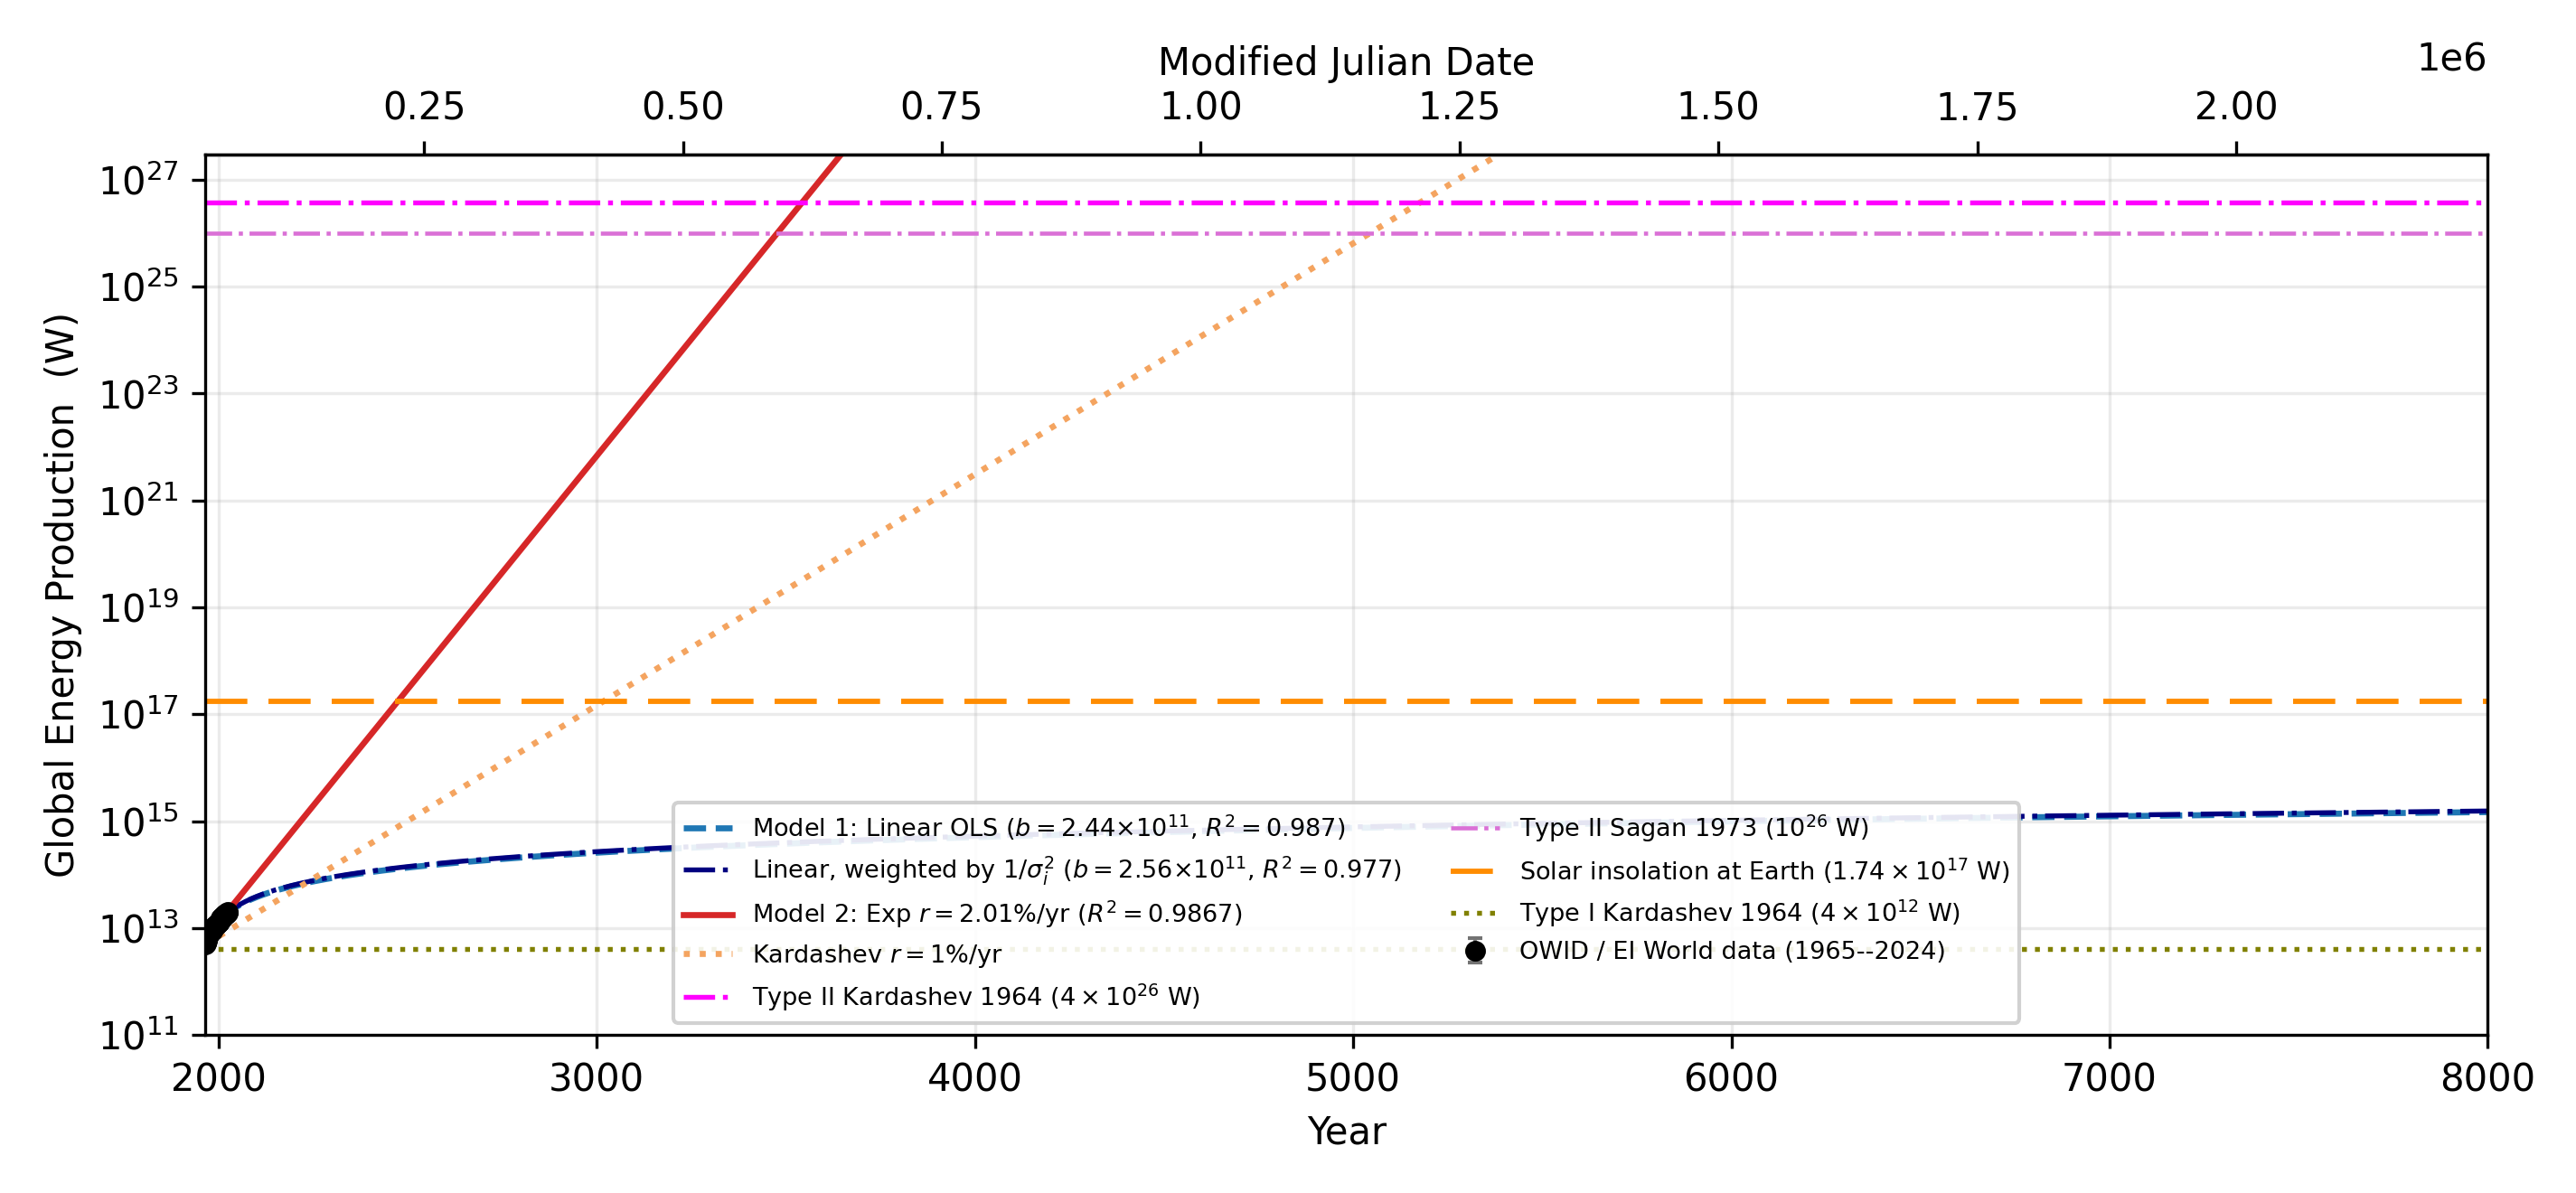
\includegraphics[width=\linewidth]{figures/fig1_energy_loglog.png}
% --- error bars are the adopted heteroscedastic model (Sec. 3.3); both the
%     unweighted (OLS) and $1/\sigma_i^2$-weighted linear fits are shown. The
%     figure is produced by make_errorbar_figures.py on the OWID data. ---
\caption{Global energy production 1965--2024 (OWID direct-method dataset) in watts
(filled circles), with the unweighted best-fit linear model (Model~1, blue dashed;
$b=2.44\times10^{11}$~W~yr$^{-1}$, $R^2=0.987$), the $1/\sigma_i^2$-weighted linear fit
(navy dash-dot; $b=2.56\times10^{11}$~W~yr$^{-1}$, $R^2=0.977$), the free-rate exponential
fit (Model~2, red solid; $r=2.01\%~\mathrm{yr^{-1}}$, $R^2=0.987$), the standard Kardashev
one-percent exponential (salmon dotted), and the
Kardashev Type~I, Type~II (\citealp{Kardashev1964} and \citealp{Sagan1973}) and
solar-insolation reference levels (horizontal lines). The one-percent model diverges
visibly from the data over the full six-decade baseline. The OWID series reports point
estimates without published per-year uncertainties; we adopt a heteroscedastic error
model (Section~\ref{sec:limitations}) with fractional uncertainties declining from
$\sim5$--$10\%$ before 1980 to $\sim1$--$2\%$ after 2000, reflecting improving reporting
coverage. On this logarithmic ordinate the corresponding error bars are smaller than the
plotting symbols. Refitting under $1/\sigma_i^2$ weighting leaves every qualitative
conclusion unchanged: the one-percent Kardashev model remains decisively
rejected, and the linear and free-rate exponential models remain statistically
indistinguishable by the Widely Applicable Information Criterion
(Section~\ref{sec:mcmc}).}
\label{fig:energy_loglog}
\end{figure}

\subsection{The Linear Model: an Excellent Fit with a Physical Reductio}
\label{sec:linear}

We next consider a linear OLS model
\begin{equation}
\label{eq:linear}
P_L(t) = a + b\,t,
\end{equation}
with parameters $a$ and $b$ estimated by minimising the sum of squared residuals.
Following Occam's razor \citep{Blumer1987}, this two-parameter model is the simplest
physically plausible alternative. The OLS solution gives
$b=2.44\times10^{11}~\mathrm{W\,yr^{-1}}$ and coefficient of determination $R^2=0.987$.
The fit is excellent over the six-decade baseline of the data
(Figure~\ref{fig:energy_loglog}). Figure~\ref{fig:energy_linear} shows the same data and
fits on a linear vertical axis, making the remarkably low dispersion directly visible:
the linear and exponential models are visually near-identical across 1965--2024, while
the Kardashev one-percent model diverges strikingly downward from the data.

\begin{figure}[htbp]
\centering
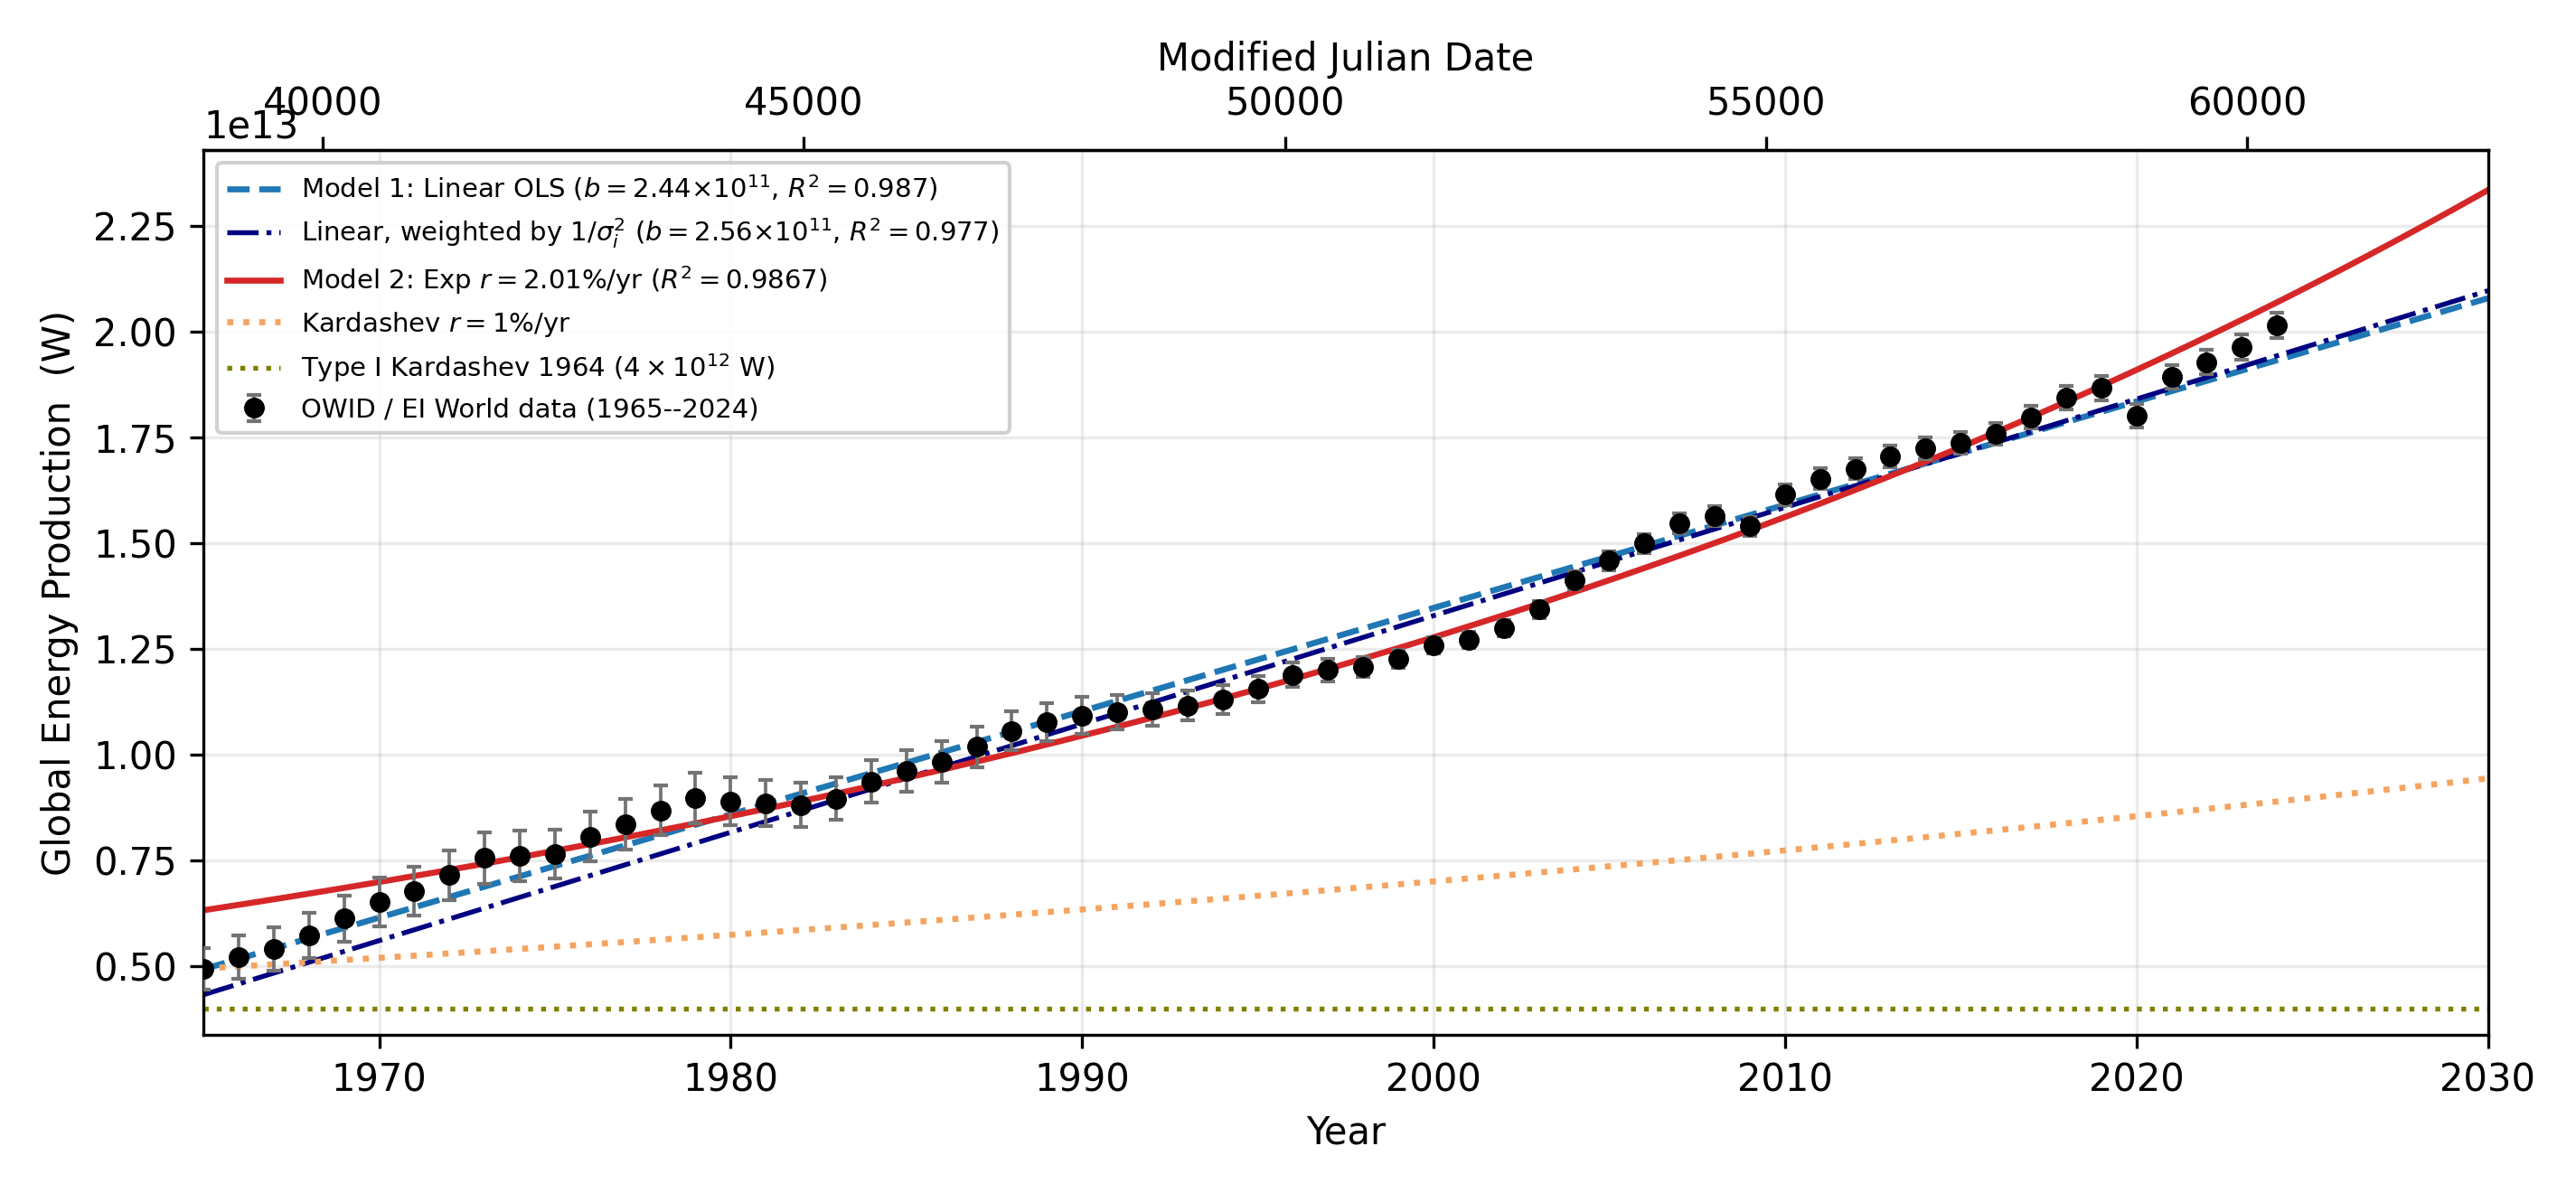
\includegraphics[width=\linewidth]{figures/fig2_energy_linear.png}
\caption{Re-scaled version of the OWID global primary-energy data (1965--2024) on a linear
vertical axis (W), with the unweighted linear OLS fit (blue dashed,
$b=2.44\times10^{11}$~W~yr$^{-1}$, $R^2=0.987$), the $1/\sigma_i^2$-weighted linear fit
(navy dash-dot, $b=2.56\times10^{11}$~W~yr$^{-1}$, $R^2=0.977$), and the free-rate
exponential fit ($r=2.01\%~\mathrm{yr^{-1}}$; red solid, $R^2=0.987$). The two linear fits
and the exponential are visually near-identical over the six-decade baseline, confirming
the WAIC result that the functional forms are statistically indistinguishable on the
observed data. Vertical error
bars show the adopted per-year uncertainties (Section~\ref{sec:limitations}): comparable
to or smaller than the marker size for post-2000 data and growing to $\sim5$--$10\%$ for
the earliest points. The Kardashev one-percent exponential (salmon dotted) diverges
dramatically downward from the data, falsifying the conservative assumption universally
adopted in the subsequent literature. The weighting raises the
linear slope by $\approx5\%$ (from $b=2.44\times10^{11}$ to $2.56\times10^{11}$~W~yr$^{-1}$),
as the higher-uncertainty early points are down-weighted, but does not alter the WAIC model
preference of Section~\ref{sec:mcmc} or the order-of-magnitude Type~II timescale; the
Shapiro--Wilk non-Gaussianity
(Figure~\ref{fig:deltaP}) is driven by the well-measured 2008 and 2020 outliers and is
insensitive to the early-decade weighting. The Kardashev Type~I threshold from 1964
($4\times10^{12}$~W) lies well below the full dataset: Earth has long since surpassed
Kardashev's original Type~I energy benchmark.}
\label{fig:energy_linear}
\end{figure}

To assess the normality of the residual structure, we compute the year-over-year
absolute differences $\Delta P_i = P_i - P_{i-1}$ and apply the Shapiro--Wilk normality
test \citep{ShapiroWilk1965}. We obtain $W=0.925$, $p=0.0014$: we reject the null
hypothesis that $\Delta P$ is drawn from a Normal distribution. The distribution of
$\Delta P$ (Figure~\ref{fig:deltaP}) exhibits significant negative skewness
(skewness $=-0.664$), driven by identifiable exogenous shocks to global energy
production at 2008 (subprime financial crisis) and 2020 (COVID-19 pandemic). This
non-Gaussian structure constitutes direct evidence of path-dependence in the global
energy system: large negative shocks are systematically more probable than an
independent-increment multiplicative generator with positive drift would predict, and
their occurrence is traceable to specific historical events rather than symmetric
statistical fluctuations.

\begin{figure}[htbp]
\centering
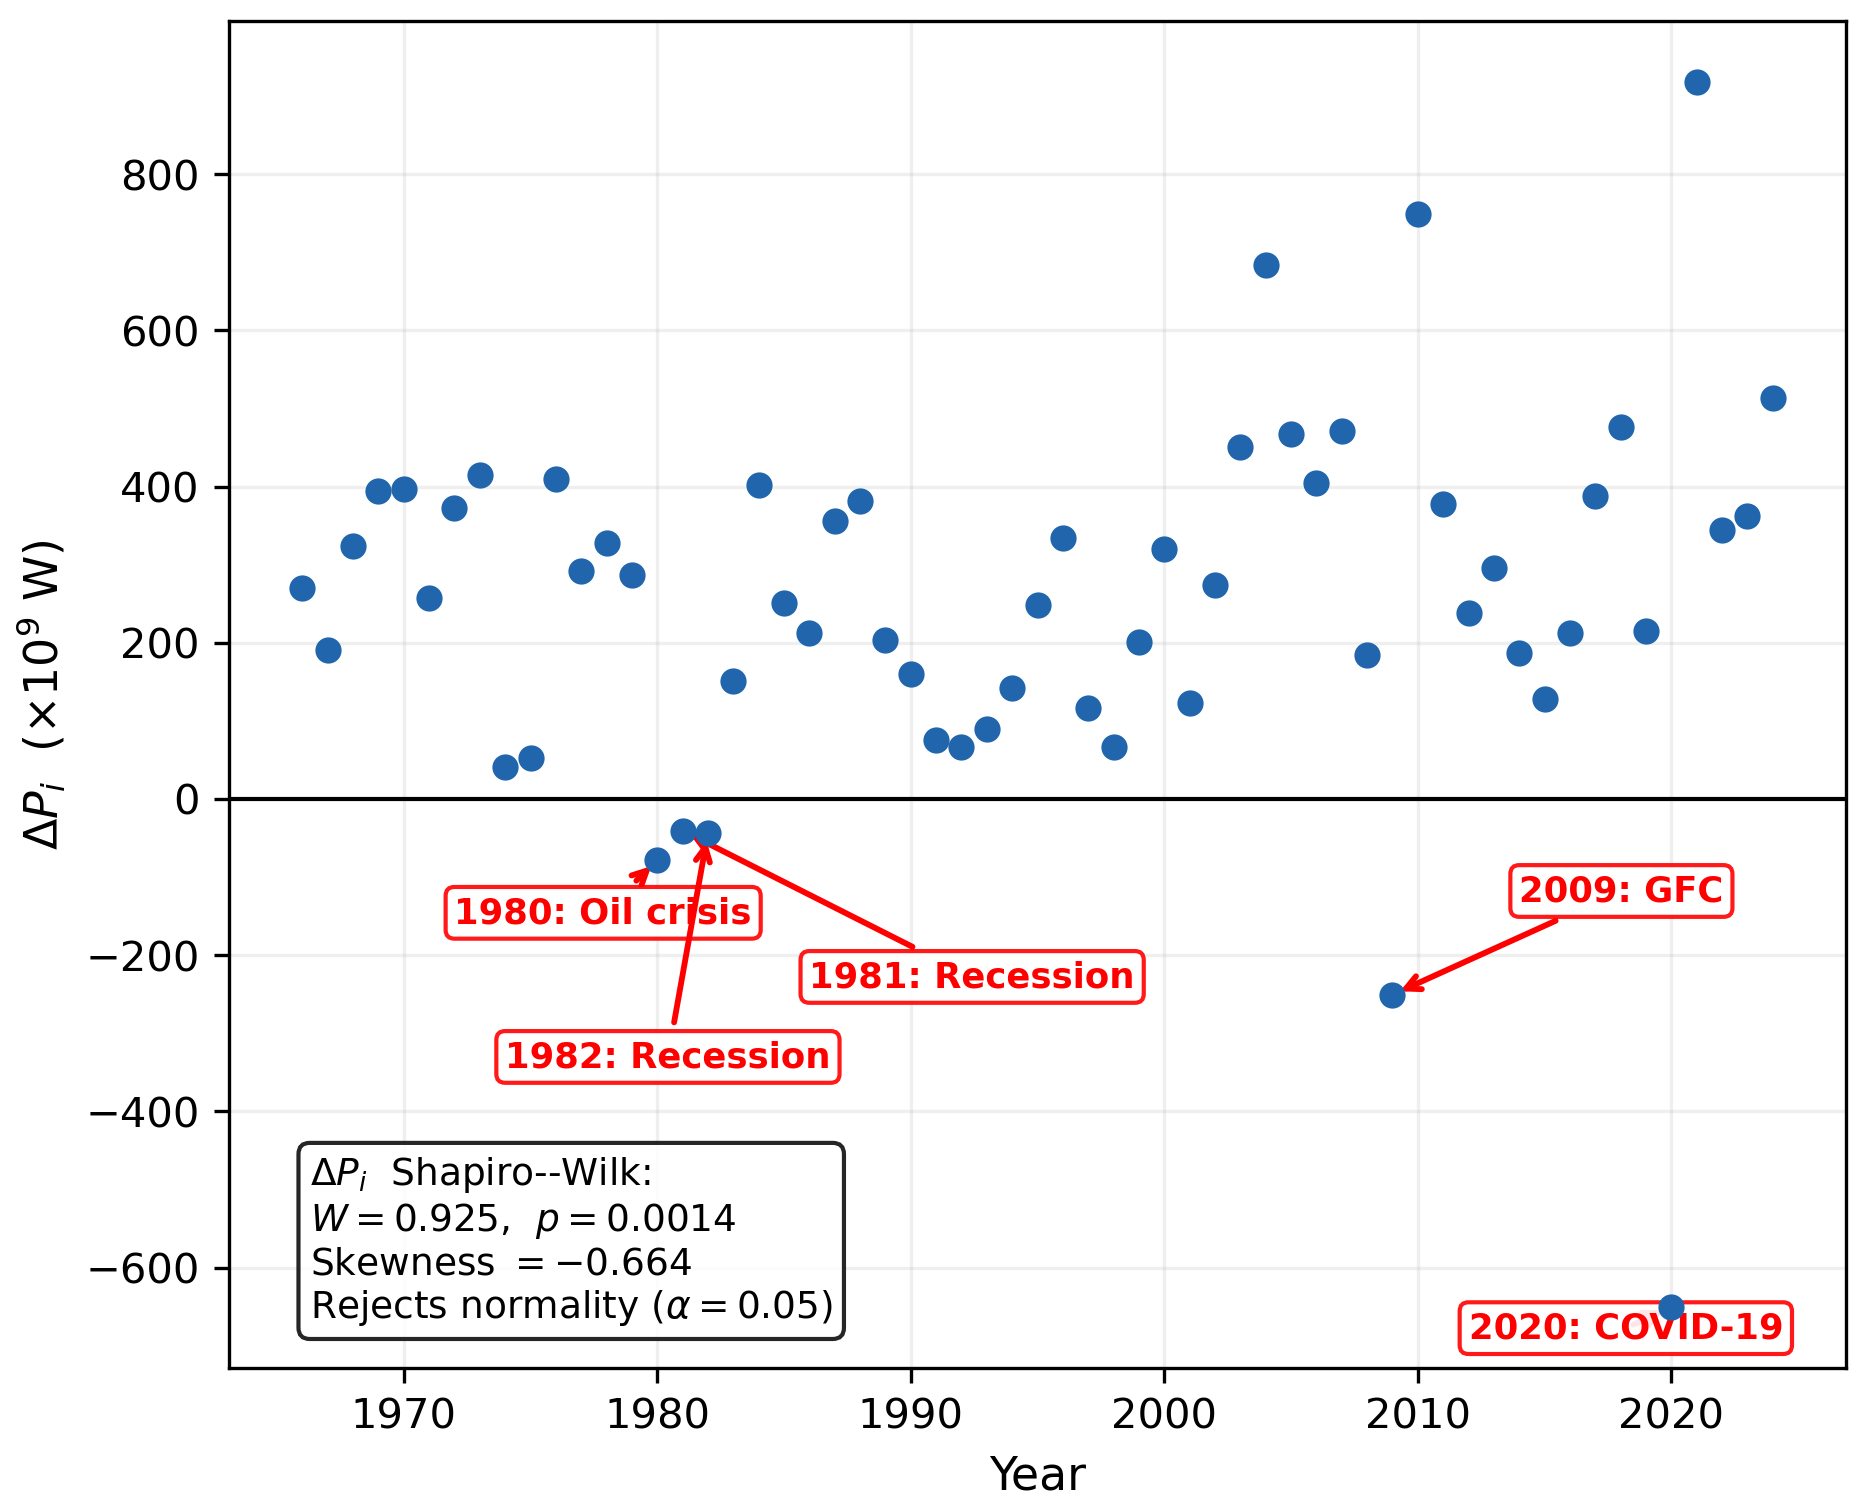
\includegraphics[width=0.85\linewidth]{figures/fig3_deltaP.png}
\caption{Year-over-year increments $\Delta P_i = P_i - P_{i-1}$ in global energy
production (1966--2024), in units of $10^9$~W. The distribution is significantly
non-Gaussian (Shapiro--Wilk $W=0.925$, $p=0.0014$) and negatively skewed
(skewness $=-0.664$). The largest negative excursions coincide with identifiable
historical shocks --- the 1980--1982 oil crisis and recessions, the 2009 global
financial crisis, and the 2020 COVID-19 pandemic --- demonstrating path-dependence
inconsistent with the independent-increment structure of a geometric growth series.
These well-measured, recent-decade outliers dominate the non-Gaussian signal and are
insensitive to the early-decade uncertainty weighting discussed in
Section~\ref{sec:limitations}. Error bars are deliberately not drawn on $\Delta P$: the
adopted per-year uncertainties (Section~\ref{sec:limitations}) are dominated by systematic
effects --- accounting conventions, reporting coverage, retroactive harmonisation --- that
are strongly correlated between adjacent years and therefore cancel in the difference
$P_i-P_{i-1}$. Independent propagation of the full per-year uncertainty would overstate the
error on $\Delta P$ by a large factor (yielding bars comparable to the increments
themselves) and is inappropriate here; the year-to-year change in global energy is in fact
constrained far more tightly than the absolute level.}
\label{fig:deltaP}
\end{figure}

A further structural objection to $(1+x)^t$ with $x>0$ is that the model is
sign-constrained: every year must exhibit positive growth by construction. The observed
series contains identifiable years of negative growth (e.g.\ 2008 and 2020) that the
model cannot accommodate at any parameter value --- a structural, not merely statistical,
falsification of the always-positive growth assumption that is independent of the
non-Gaussianity and path-dependence arguments above.

Notwithstanding its excellent in-sample fit, the linear model fails catastrophically on
extrapolation. Solving $P_L(t^\ast)=L_\odot$ gives
\begin{equation}
\label{eq:textrap}
t^\ast = \frac{L_\odot - a}{b} \approx 1.6\times10^{15}~\mathrm{yr}
\approx 1.2\times10^{5}\,H_0^{-1},
\end{equation}
where $H_0^{-1}\approx13.8$~Gyr is the Hubble time. The implied Type~II timescale exceeds
the age of the Universe by five orders of magnitude. This is not merely improbable --- it
is physically incoherent, since it vastly exceeds the main-sequence lifetime of the Sun
and the projected heat death of the Universe. We designate this result Kardashev's
Conundrum: the linear model, which best fits the data by all standard statistical
criteria, predicts a civilisational transition timescale that is cosmologically
nonsensical.

\subsection{Model Comparison via MCMC and WAIC}
\label{sec:mcmc}

To place the comparison on a rigorous Bayesian footing, we fit an exponential model with
the growth rate $r$ as a free parameter,
\begin{equation}
\label{eq:exp}
P_E(t) = a_0\, e^{rt},
\end{equation}
using a Metropolis--Hastings Markov Chain Monte Carlo (MCMC) sampler
\citep{Metropolis1953,Hastings1970} with a prior $r\sim\mathcal{N}(0.01, 0.02^2)$ centred
on the Kardashev value and $N=60{,}000$ posterior samples after a $15{,}000$-step
burn-in. The burn-in phase is discarded because the first iterations of the chain are
influenced by the arbitrary starting point in parameter space rather than by the target
posterior; the Markov property of the sampler ensures that the chain eventually forgets
this initial condition and converges to the stationary distribution, from which the
retained samples are drawn. The posterior mean growth rate is
$r=2.01\%\pm0.03\%~\mathrm{yr^{-1}}$ (95\% credible interval $[1.94\%, 2.08\%]$), with
the Kardashev value of $1\%~\mathrm{yr^{-1}}$ lying well outside the 95\% credible
interval. The best-fit exponential model gives $R^2=0.987$, nearly identical to the
linear model ($\Delta R^2 < 0.001$).

Two cautions attach to the precision of this interval. First, it is derived from a single
realisation --- the energy trajectory of one civilisation --- and therefore quantifies the
sampling uncertainty \emph{within} our own history, not the inaccessible dispersion of
growth rates across the population of civilisations that the Kardashev framework ultimately
concerns. Ours is, for now, the only example on which to base a Kardashev law. Second, even
within this single trajectory the annual observations are not independent: the year-on-year
increments are positively autocorrelated ($\rho_1=0.35$; Section~\ref{sec:independence})
and the residuals about the fitted trend more strongly so, so the sixty data points carry
appreciably less independent information than sixty i.i.d.\ samples would. The credible
interval quoted above, which assumes independent errors, is correspondingly optimistic, and
an autocorrelation-aware error model would widen it. Neither caution alters the qualitative
conclusions --- the one-percent rate remains decisively excluded --- but both temper any
over-literal reading of the $\pm0.03\%$ figure.

The Widely Applicable Information Criterion (WAIC; \citealp{Watanabe2010}) comparison
yields $\Delta\mathrm{WAIC} = \mathrm{WAIC}_{\mathrm{exp}} - \mathrm{WAIC}_{\mathrm{linear}} = 5.5$.
The standard error of this difference, however, is large: computed from the pointwise
predictive densities, $\mathrm{SE}(\Delta\mathrm{WAIC})\approx18$, so the difference lies
well within one standard error of zero ($\Delta\mathrm{WAIC}/\mathrm{SE}\approx0.3$). The
slight numerical edge to the linear model is therefore not statistically significant: on
the observed baseline the two functional forms are statistically indistinguishable. Both
carry $K=2$ free parameters, so the AIC and BIC penalties are identical. Together, the
near-identical $R^2$ values ($\Delta R^2<0.001$) and the consistency of
$\Delta\mathrm{WAIC}$ with zero confirm the statistical statement of Kardashev's Conundrum:
the data cannot distinguish between the two functional forms on the observed baseline, so
the choice of which functional form to extrapolate is underdetermined by the fit --- yet
the linear form, an entirely adequate description, implies a cosmologically absurd Type~II
timescale (Eq.~\ref{eq:textrap}).

The complete statistical picture is:
\begin{enumerate}
\item The one-percent Kardashev exponential is falsified by the data (poor fit; posterior
$r=2.01\%$, well outside the one-percent prior).
\item The linear model and the free-$r$ exponential have statistically identical
in-sample performance ($\Delta R^2 < 0.001$) and are statistically indistinguishable by
WAIC ($\Delta\mathrm{WAIC}=5.5$, with $\mathrm{SE}(\Delta\mathrm{WAIC})\approx18$).
\item The year-over-year differences $\Delta P$ are non-Gaussian (Shapiro--Wilk
$W=0.925$, $p=0.0014$), exhibiting path-dependent negative skewness inconsistent with any
independent-increment multiplicative generator with positive drift.
\item The linear model is physically falsified by extrapolation (Type~II timescale
$\sim1.2\times10^{5}\,H_0^{-1}$).
\end{enumerate}
No functional form fitted to $P(t)$ can simultaneously satisfy statistical adequacy and
physical coherence. The two data-adequate descriptions fail for complementary reasons: the
linear model reaches the Type~II threshold only after a cosmologically absurd
$\sim10^5$ Hubble times (Eq.~\ref{eq:textrap}), while the free-$r$ exponential, though it
would reach the threshold in $\sim3500$~yr, is excluded as a \emph{sustained} trajectory on
physical grounds. Exponential energy growth is self-terminating: the accompanying waste
heat renders an Earth-like planet uninhabitable within $\lesssim10^3$~yr
(\citealp{BalbiLingam2025}; see Section~\ref{sec:technosignatures}), and, more generally,
growth within any finite resource base must saturate, the exponential being merely the
early-time limit of bounded (logistic) dynamics. The choice of functional form is therefore
immaterial: neither yields a physically coherent path to the energy-scaling Type~II
threshold. This is the Conundrum, stated precisely.

\subsection{The KSN Resolution: Renormalisation to $\mathrm{J\,Hash^{-1}}$}
\label{sec:ksn}

The resolution of Kardashev's Conundrum cannot be achieved by selecting a different
fitting function for the same state variable $P(t)$, because the problem is not one of
functional form --- it is one of variable choice. We demonstrate this via the following
argument.

\paragraph{Dimensional incompleteness} The Kardashev scale measures energy throughput,
$P\,[\mathrm{W}=\mathrm{J\,s^{-1}}]$, but makes no reference to what that energy
accomplishes. As \citet{Sagan1973} noted, a civilisation that wastes energy inefficiently
is rated equally to one that channels the same power into information-rich computation.
The scale is therefore dimensionally incomplete as a measure of civilisational
advancement: it conflates energy expenditure with technological capability.

\paragraph{The Landauer connection} The fundamental physical link between energy and
information is the Landauer limit \citep{Landauer1961,Bennett1982}: the minimum energy
required to erase one bit of information at temperature $T$ is
$k_B T \ln 2 \approx 2.85\times10^{-21}$~J at room temperature. The ratio $P/H$ --- global energy production divided by the global \emph{proof-of-work}
hashrate --- has dimensions of energy per hash, and is an empirical measure of how
efficiently a civilisation converts energy into irreversible computational work. A single
hash is not a single bit erasure: evaluating a double SHA-256 hash entails a large,
hardware- and algorithm-dependent number $N_b$ of irreversible bit operations, so the
thermodynamic floor on $B=P/H$ is not the Landauer bound itself but a multiple of it,
$B_{\min}=N_b\,k_B T\ln 2$, lying many orders of magnitude above
$k_B T\ln 2\approx2.85\times10^{-21}$~J. As $B$ approaches this per-hash floor a
civilisation approaches the thermodynamic limit of its computation. Our physical variable
thus inherits physical meaning absent from $P(t)$ alone.

\paragraph{The renormalisation} We define the KSN state variable as
\begin{equation}
\label{eq:ksn}
B(t) = \frac{P(t)}{H(t)}\quad [\mathrm{J\,Hash^{-1}}] \equiv \mathrm{KN},
\end{equation}
where $H(t)$ is the yearly average Bitcoin network hashrate in $\mathrm{Hash\,s^{-1}}$.
We use the Bitcoin hashrate because it is the only publicly auditable, unforgeable, and
continuously updated global record of proof-of-work computation \citep{Nakamoto2009},
fulfilling the requirement of \citet{Sagan1973} that the Kardashev state variable be
sensitive to the ``security of vast quantities of information.'' The \emph{choice} of this
denominator is a modelling decision rather than a forced one --- other normalisations
(global FLOPS, total computing energy) would yield different trajectories, as discussed in
Section~\ref{sec:limitations} --- but once the denominator is fixed the renormalisation
introduces no fitted parameter, being a ratio of two independently measured physical
quantities.

\paragraph{Statistical motivation} The variable transformation $P \to B = P/H$ is not a
Box--Cox power transformation of $P$ \citep{BoxCox1964}, which would remain within the
family of functional forms fitted to the original variable. It is instead a ratio
normalisation by an external physically motivated quantity, taking the analysis outside
the Box--Cox family. The KSN variable $B(t)$ is our proposal for the correct extensive
variable of the Kardashev scale.

\paragraph{Concurrent work} Complementary work from the quantum-computing perspective
has recently examined Bitcoin mining as a Kardashev-scale problem
\citep{DallaireDemers2026}, demonstrating that quantum-accelerated Bitcoin mining at
current network difficulty would require a fleet of $\sim10^{23}$ physical qubits drawing
$\sim10^{25}$~W --- resources consistent with a Kardashev Type~II civilisation. Their
result places an upper bound on quantum-mining feasibility: the resource requirements are
so extreme that practical quantum mining collapses under hardware, error-correction, and
fleet-logistics overheads. Our analysis is methodologically distinct --- we use the
Bitcoin hashrate as an empirical proxy for global classical proof-of-work and renormalise
the Kardashev state variable accordingly --- but shares the use of proof-of-work
infrastructure as a natural bridge between civilisational energy and irreversible
computation.

\paragraph{Adjacent technosphere literature} A parallel research programme has
approached the limits of civilisational growth from the perspective of technosignatures
and technosphere modelling. \citet{Wright2022} synthesise the longstanding SETI-community
argument that technosignatures may be more abundant, longer-lived, and more detectable
than biosignatures, motivating renewed interest in quantitative frameworks for
civilisational scale. \citet{HaqqMisra2025a} developed ten self-consistent scenarios for
Earth's technosphere over a thousand-year horizon --- three with zero-growth stability,
two that have collapsed, one that oscillates, and four that continue to grow ---
illustrating that conventional Kardashev-style continuous-growth extrapolation captures
only a subset of plausible long-term futures. \citet{HaqqMisra2025b} argue that the
Kardashev scale is better understood as a ``luminosity limit'' --- the maximum capacity
for a civilisation to harvest luminous stellar energy within a given spatial domain ---
and that thermodynamic efficiency keeps any luminosity-limited technosphere strictly
below this theoretical maximum. \citet{BalbiLingam2025} analyse, via simple thermodynamic
models, the constraints that unavoidable waste-heat generation imposes on the long-term
habitability of Earth-like planets hosting technospheres in persistent exponential
growth, demonstrating that the loss of habitable surface conditions can be expected on
timescales of $\lesssim10^3$~yr from the onset of the exponential phase, for an assumed
annual energy-consumption growth rate of $\sim1\%$ --- the same conservative Kardashev
rate that the present work statistically falsifies. \citet{Cirkovic2018} situates such
constraints within a four-category taxonomy of Fermi-paradox solutions, whose
``logistic'' category groups hypotheses in which Galactic sophonts exist and are in
principle detectable but the cost of maintaining detectability over astrophysical
timescales is prohibitive. We draw these threads together in
Section~\ref{sec:technosignatures}, where the falsification of
Section~\ref{sec:standard}--\ref{sec:mcmc} is shown to supply a specific, data-driven
mechanism within that logistic category.

Figure~\ref{fig:ksn} shows $B(t)$ for 2009--2024, spanning 16 annual data points and 14
orders of magnitude in $B$. Because $P(t)$ varies by only $\sim30\%$ over this window while
$H(t)$ grows by fourteen orders of magnitude, $B=P/H$ is numerically dominated by the
hashrate denominator: to within the slowly varying energy prefactor, $B(t)$ is the inverse
of the global proof-of-work hashrate and traces the history of proof-of-work energy
efficiency. The data display a steeply decreasing trend reflecting the rapid improvement in
Bitcoin proof-of-work energy efficiency from the CPU era (2009) through the GPU era
(2010--2012) to the ASIC era (2013--2024). The structural breaks
between these eras preclude a single-exponential description of $B(t)$; a formal
era-segmented functional fit is deferred to a future paper.

\begin{figure}[htbp]
\centering
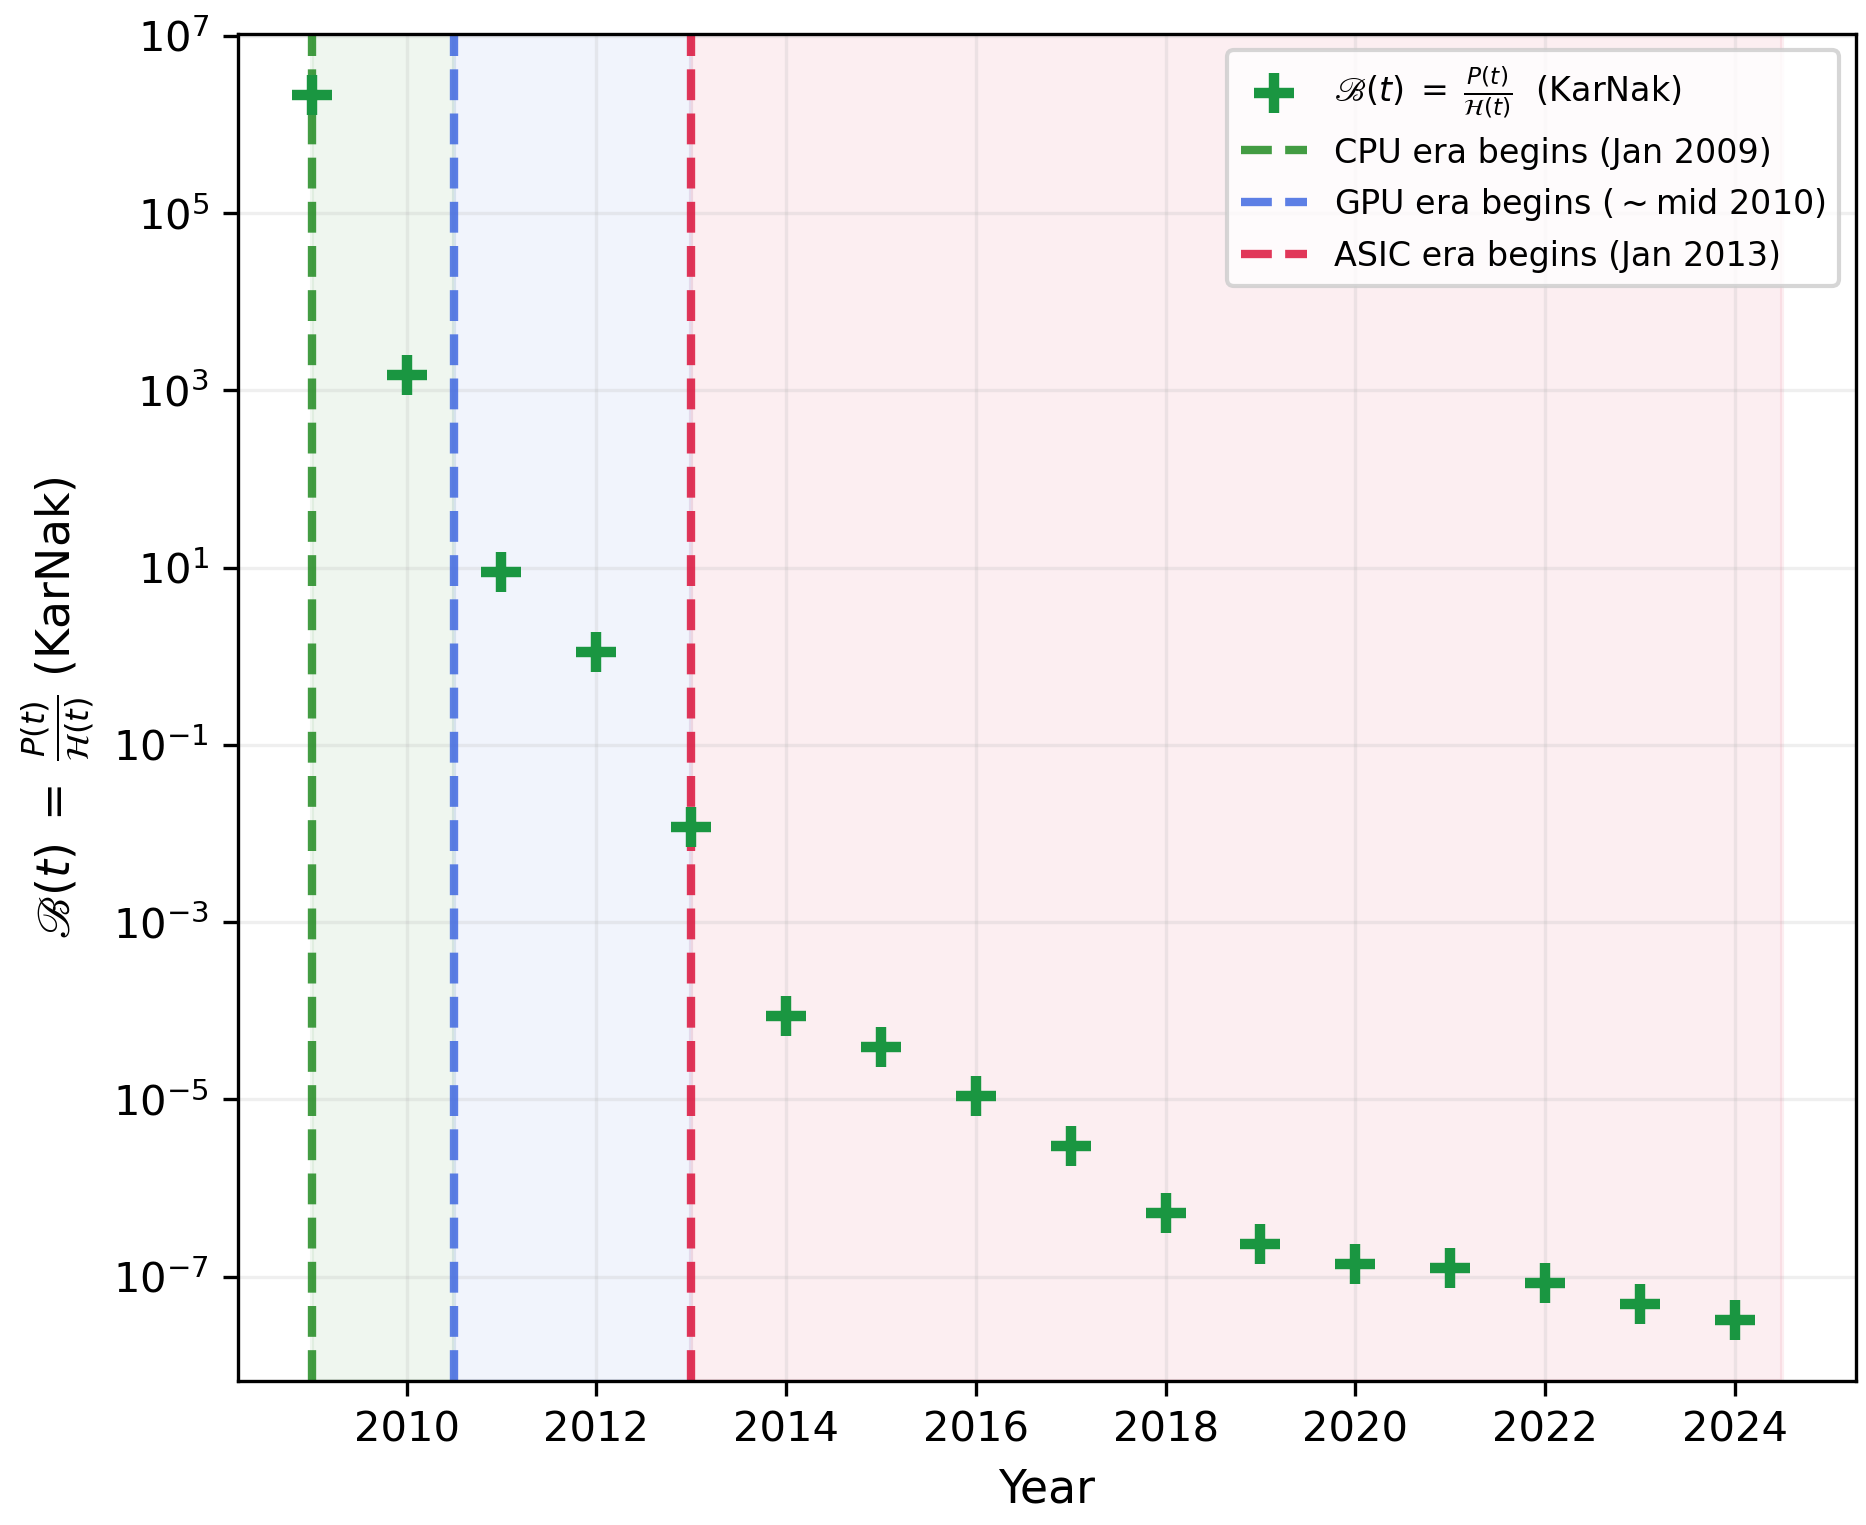
\includegraphics[width=0.8\linewidth]{figures/fig4_ksn.png}
\caption{The KSN state variable $B(t)=P(t)/H(t)$ in KarNak units ($\mathrm{J\,Hash^{-1}}$)
for 2009--2024, spanning 14 orders of magnitude. The steeply decreasing trend
reflects the rapid improvement in Bitcoin proof-of-work energy efficiency from the CPU
era (2009) through the GPU era (2010--2012) to the ASIC era (2013--2024). Structural
breaks between eras preclude a single-exponential description; a formal fit is deferred
to a future paper. The largest uncertainties attach to the 2009--2013 CPU/GPU-era points,
whose annual-average hashrates are derived from the on-chain difficulty record
(Section~\ref{sec:data}) rather than measured directly; on this fourteen-decade
logarithmic ordinate, however, even these uncertainties are smaller than the plotting
symbols, so error bars are not shown.}
\label{fig:ksn}
\end{figure}

\subsection{Civilisational Timescales on the KSN Scale}
\label{sec:timescales}

Table~\ref{tab:timescales} summarises the Type~II timescales implied by each model. The
Kardashev and Sagan exponential models give timescales of order $10^3$~yr. These are
reached tautologically: any exponential model of the form $P=P_0 e^{rt}$ will reach any
finite threshold at some finite time, so the Type~II crossing year is determined by the
assumed growth rate $r$ and is not a prediction in any falsifiable sense. The linear
model, as shown in Eq.~(\ref{eq:textrap}), gives a timescale that is cosmologically
absurd. On the KSN scale, the concept of a Type~II threshold must be re-expressed in
terms of $B=P/H$: a Type~II KSN civilisation is one for which $B$ approaches its thermodynamic
floor, i.e.\ the energy cost per hash approaches the per-hash Landauer limit
$N_b\,k_B T \ln 2$ (a hardware-dependent multiple of the single-bit bound). This reframing is
consistent with the original intent of \citet{Kardashev1964} and the
information-theoretic extension proposed by \citet{Sagan1973}.

\begin{table}[htbp]
\centering
\caption{Type~II civilisation timescales under each model. All timescales are measured
from 1964. $H_0^{-1}=13.8$~Gyr is the Hubble time. The MCMC exponential uses the
posterior mean $r=2.01\%~\mathrm{yr^{-1}}$.}
\label{tab:timescales}
\begin{tabular}{@{}llll@{}}
\hline
Model & Growth rate & Type~II year (CE) & $\Delta t/H_0^{-1}$ \\
\hline
Kardashev 1964 (fixed $r$)   & $1.00\%~\mathrm{yr^{-1}}$            & $\sim 5188$           & $\sim 2\times10^{-7}$ \\
Exp.\ free $r$ (MCMC mean)   & $2.01\%~\mathrm{yr^{-1}}$            & $\sim 3547$           & $\sim 1\times10^{-7}$ \\
Linear OLS                   & $2.44\times10^{11}~\mathrm{W\,yr^{-1}}$ & $\sim 1.6\times10^{15}$ & $\sim 1.2\times10^{5}$ \\
KSN ($B=P/H$)                & $B\to N_b\,k_B T\ln 2$                    & \multicolumn{2}{l}{Re-expressed via Landauer limit} \\
\hline
\end{tabular}
\end{table}

\begin{table}[htbp]
\centering
\caption{Comparison of energy-production baselines and Type~II civilisation timescale
predictions. $P_0$ is the average continuous power at the start of each analysis,
converted from the reported annual energy via Eq.~(\ref{eq:conv}). $H_0^{-1}=13.8$~Gyr is
the Hubble time.}
\label{tab:baselines}
\begin{tabular}{@{}lll@{}}
\hline
Source & $P_0$ & Type~II timescale \\
\hline
\citet{Kardashev1964} (1964 estimate)        & $4.00$~TW & $\sim 3.2$~kyr at $r=1\%~\mathrm{yr^{-1}}$ \\
OWID \citep{Ritchie2022} (1965, this work)   & $4.95$~TW & $\sim 1.2\times10^{5}\,H_0^{-1}$ (linear OLS) \\
\hline
\end{tabular}
\end{table}

\subsection{The Independence Property as a Further Objection to the Exponential}
\label{sec:independence}

A complementary objection arises from the theory of stochastic processes. The deterministic
series $P(t)=P_0(1+x)^t$ is the mean path of a multiplicative process $P_t=G_t\,P_{t-1}$
whose annual growth factors $G_t$ have mean $1+x$. The model's essential structural
assumption is that the $\{G_t\}$ are independent and identically distributed; equivalently,
the log-increments $\xi_t\equiv\ln(P_t/P_{t-1})$ are i.i.d., so that $\ln P_t$ is a random
walk with constant drift. Such a process is \emph{memoryless} in the precise sense that,
conditional on the present, the next increment is independent of the entire history that
produced it:
\begin{equation}
\label{eq:memoryless}
\Pr\!\left(\xi_{t+1}\le z \,\middle|\, \xi_t,\xi_{t-1},\dots,\xi_1\right)
   = \Pr\!\left(\xi_{t+1}\le z\right).
\end{equation}
The model thus embeds no channel through which the trajectory's past can shape its future
beyond fixing the current level.\footnote{This process-level memorylessness is the
stochastic-process counterpart of the memoryless property $P(X>a+b\mid X>b)=P(X>a)$, which
\emph{uniquely} characterises the geometric distribution among discrete laws and the
exponential among continuous ones; in both settings the defining feature is that the past
conveys no information about the future. Memorylessness is therefore a highly exceptional
property --- any system that learns, accumulates capital, or is scarred by its own history
carries memory by default.}

Civilisational energy systems are not memoryless in this sense. Infrastructure lock-in,
capital-stock inertia, technology-diffusion dynamics, geopolitical constraints, and the
persistent after-effects of crises all make the current increment depend on the path taken
to reach the present state. Three independent empirical signatures contradict the
i.i.d.-increment hypothesis. First, the growth factors are serially dependent: the lag-one
autocorrelation of $\xi_t$ is $\rho_1=0.35$, and a Ljung--Box test rejects serial
independence at every lag from one to four ($Q=7.8$--$12.8$, $p<0.02$; Durbin--Watson
$=1.25$; runs-test $z=-2.5$, $p=0.014$). Growth is positively autocorrelated --- expansions
and contractions each cluster in time --- which is the direct signature of memory and is
incompatible with independent increments. Second, the increment distribution is
significantly non-Gaussian and negatively skewed (Shapiro--Wilk $W=0.925$, $p=0.0014$;
skewness $-0.664$; Figure~\ref{fig:deltaP}), with the heaviest negative excursions
traceable to identifiable exogenous shocks (2008, 2020) rather than to symmetric random
draws. Third, and most simply, the series contains years of outright negative growth
(e.g.\ 2009, 2020), which the strictly increasing model $(1+x)^t$ with $x>0$ cannot
represent at any parameter value. The independence property is therefore not an abstract
technicality but a testable claim about the generative process, and on three independent
measures the evidence is against it: the energy trajectory of a civilisation carries
memory, and a memoryless multiplicative generator cannot reproduce it.

Before discussing falsifiability and limitations, we note the most immediate consequence
of the foregoing analysis. Because observed energy growth is sub-exponential, the
energy-scaling Type~II threshold is unreachable on any physically coherent timescale
(Eq.~\ref{eq:textrap}); the corollary --- that Type~II energy-harvesting technosignatures
such as Dyson spheres are unlikely to arise on the energy trajectory we observe, and so
offer a candidate physical explanation for their continued non-detection --- is, we argue,
the principal observational result of this work, and we treat it in full in
Section~\ref{sec:technosignatures}.

% =====================================================================
\section{Discussion}
\label{sec:discussion}

\subsection{A Physical Explanation for the Non-Observation of Type~II Technosignatures}
\label{sec:technosignatures}

The statistical results of Section~\ref{sec:analysis} carry a direct and, to our
knowledge, previously unquantified consequence for SETI. We state it at the head of the
discussion because it is the result most likely to be of interest to the observational
technosignature community, and because it follows from the falsification rather than from
any additional assumption.

Over the six-decade observed baseline, global energy production is sub-exponential. The
one-percent geometric model is rejected outright (Section~\ref{sec:standard}); the data
are described equally well by a linear model and a free-rate exponential at
$r\approx2\%~\mathrm{yr^{-1}}$, statistically indistinguishable by WAIC
($\Delta\mathrm{WAIC}=5.5$, well within its standard error; Section~\ref{sec:mcmc}). On the linear description, the
energy-scaling Type~II threshold $P\to L_\odot$ is reached only after
$t^\ast\approx1.6\times10^{15}~\mathrm{yr}\approx1.2\times10^{5}\,H_0^{-1}$
(Eq.~\ref{eq:textrap}) --- a timescale that exceeds the main-sequence lifetime of the
host star by some five orders of magnitude. The implication is not merely that Type~II is
distant: it is that the star a Dyson sphere would enclose evolves off the main sequence,
exhausts its hydrogen, and is gone long before any civilisation growing its energy budget
at the observed rate could approach that star's luminosity. The energy-scaling Type~II
threshold is, in this sense, not a destination on the civilisation's trajectory at all. A
Type~II energy-harvesting technosignature --- a Dyson sphere, or any equivalent
full-luminosity collector --- is therefore unlikely to be a common, persistent feature of
the Galaxy.

This furnishes a physical, data-driven explanation for the outcome of the observational
Dyson-sphere search programme. The IRAS whole-sky upper limit of \citet{Carrigan2009},
the $\hat{G}$ infrared search of \citet{Wright2014}, and the Gaia--2MASS--WISE candidate
search of \citet{Suazo2024} have each returned no confirmed Type~II technosignature. Such
null results are conventionally attributed to the rarity of civilisations, the transience
of the Type~II phase, or the sensitivity limits of the surveys. Our analysis adds a more
elementary possibility: that the search target itself --- a structure defined by
full-stellar-energy scaling --- corresponds to a civilisational state that no technosphere
on a physically realistic energy trajectory ever attains.

This conclusion was anticipated, on qualitative grounds, by \citet{Ivanov2020}, who
argued that present-day searches are tuned to find only civilisations that share our own
``more-is-better'' growth philosophy, and that the failure of Dyson-sphere searches may
indicate the inadequacy of that philosophy rather than an empty Galaxy. The present work
supplies the missing quantitative step: a direct statistical falsification, against the
observed energy record, of precisely the unbounded-exponential assumption on which the
energy-scaling Type~II target depends.

Within the four-category taxonomy of Fermi-paradox solutions of \citet{Cirkovic2018},
this result belongs to the ``logistic'' category --- civilisations exist and are in
principle detectable, but the cost of attaining or sustaining a given detectable state
over astrophysical timescales is prohibitive. What is striking is that three logically
independent arguments now converge on the same conclusion for energy-scaling Type~II
states. (i)~The present statistical falsification shows that observed energy growth is
sub-exponential and that the Type~II threshold is correspondingly unreachable in time.
(ii)~The waste-heat habitability constraint of \citet{BalbiLingam2025} shows that
sustained exponential growth at the very $\sim1\%$ rate Kardashev assumed would render an
Earth-like planet uninhabitable within $\lesssim10^3$~yr --- destroying the civilisation,
by overheating, long before Type~II could be reached. (iii)~The luminosity-limit argument
of \citet{HaqqMisra2025b} shows that thermodynamic efficiency holds any
luminosity-limited technosphere strictly below the full-stellar-luminosity ceiling. The
first argument is statistical, the second ecological-thermodynamic, the third
efficiency-thermodynamic; their mutual independence is precisely what makes their
agreement significant. The canonical energy-scaling Type~II civilisation is disfavoured
whether one reasons from the data, from planetary habitability, or from the thermodynamics
of energy capture.

Two caveats bound this inference, and we state them plainly. First, it rests on a single
civilisation observed over a single six-decade window; we cannot exclude growth regimes
that would restore exponential scaling --- a future technological transition, or expansion
beyond the home planet onto a stellar or interstellar resource base --- and
\citet{HaqqMisra2025a} explicitly construct self-consistent thousand-year futures in
which growth continues. Second, the claim is specific to energy-scaling technosignatures:
it places no constraint on technosignatures defined along other axes, such as directed
radio or optical emission, atmospheric industrial products, or the information-theoretic
signatures implied by the KSN variable. What the convergence of three independent
arguments does establish is a shift in the burden of proof: a Galaxy-common population of
persistent Dyson spheres can no longer be treated as the natural expectation of the
Kardashev framework, but must instead be justified against three distinct physical
objections.

Finally, the unreachability of the energy-scaling Type~II threshold does not abolish the
Type~II concept; it relocates it. Under the KSN renormalisation of
Section~\ref{sec:ksn}, the Type~II milestone is re-expressed as the approach of the state
variable $B=P/H$ to its per-hash Landauer floor, $B\to N_b\,k_B T\ln 2$ (Section~\ref{sec:timescales}).
A civilisation may thus be ``Type~II'' in the information--energy sense --- performing
irreversible computation at the thermodynamic floor --- without ever enclosing a star.
The non-observation of energy-scaling Type~II technosignatures and the survival of the
Type~II concept are therefore consistent: what fails is one dimensionally incomplete
realisation of the milestone, while the scale's classificatory structure is preserved on
a state variable that real civilisations can actually traverse. This is the sense in
which the KSN model is not merely a rescaling, but a resolution of the Conundrum.

\subsection{Falsifiability of the KSN Model}
\label{sec:falsifiability}

A scientific model is meaningful only insofar as it generates predictions that can in
principle be refuted by data \citep{Blumer1987}. We identify four concrete falsification
criteria for the KSN model.

First, the posterior growth rate $r=2.01\%\pm0.03\%~\mathrm{yr^{-1}}$ is a quantitative
prediction: if sustained observation of global energy production over the coming decades
yields a growth rate consistently outside the 95\% credible interval $[1.94\%, 2.08\%]$,
the exponential component of the KSN framework is falsified.

Second, the non-Gaussian structure of $\Delta P$ (Shapiro--Wilk $W=0.925$, $p=0.0014$)
establishes that year-over-year energy increments exhibit path-dependent behaviour driven
by identifiable historical events. This is a testable claim: if future decades produce a
$\Delta P$ distribution consistent with an independent-increment multiplicative generator
with positive drift, the path-dependence argument is falsified.

Third, the KSN variable $B=P/H$ predicts a secularly decreasing trend as Bitcoin ASIC
efficiency improves toward the Landauer limit \citep{Landauer1961}. If the Bitcoin
hashrate growth stalls or reverses permanently --- for example if proof-of-work mining
becomes economically unviable --- the KSN variable would cease to decrease and the
renormalisation would lose its physical motivation. This is a genuine falsification risk
that the model acknowledges explicitly.

Fourth, the dimensional-incompleteness argument predicts that no functional form fitted to
$P(t)$ alone can resolve Kardashev's Conundrum. If a future author produces a model of
$P(t)$ without additional state variables that gives both a statistically adequate fit to
the data and a physically coherent Type~II timescale, the KSN renormalisation is
unnecessary and the argument is falsified.

\subsection{Limitations}
\label{sec:limitations}

Several limitations of the present analysis deserve explicit acknowledgement.

A methodological choice concerns the energy-accounting convention. The OWID dataset column
\texttt{primary\_energy\_consumption} reports values using the direct primary energy
method, which records the physical energy output of each source. The alternative
substitution method inflates non-fossil contributions (nuclear, hydro, wind, solar) by a
thermal efficiency factor ($\sim0.38$--$0.40$) to estimate the fossil-fuel input that
would have produced the same electricity. We adopt the direct method because the Kardashev
scale measures physical power, not fossil-fuel equivalents. We have verified that all
qualitative conclusions --- falsification of the one-percent model, preference for the
linear fit, and the persistence of the Conundrum --- hold under the substitution method,
with quantitative differences: the substitution method yields $P(1965)=7.66$~TW,
$b=3.12\times10^{11}~\mathrm{W\,yr^{-1}}$, $r=1.85\%~\mathrm{yr^{-1}}$, and a Type~II
timescale of $\sim8.9\times10^{4}\,H_0^{-1}$. The choice of accounting method does not
affect the dimensional-incompleteness argument that motivates the KSN renormalisation. We
note that the distinction between these methods will grow in significance as the global
energy mix shifts toward nuclear and renewable sources --- a transition that appears to be
accelerating, with several nations expanding nuclear capacity --- since the substitution
method increasingly overstates the total energy budget relative to the physical power
actually delivered.

A further methodological consideration concerns per-year measurement uncertainties. The
OWID dataset reports point estimates only; neither the Energy Institute nor the EIA
publishes formal per-year uncertainty bands on global primary-energy production.
Methodological considerations suggest that pre-1980 data carry larger fractional
uncertainty ($\sim5$--$10\%$) than post-2000 data ($\sim1$--$2\%$) due to incomplete
reporting coverage in earlier decades, retroactive harmonisation of accounting methods,
and imputation for missing country-year cells. To test the sensitivity of our conclusions
to this heteroscedasticity, we adopt a per-decade fractional-uncertainty model that
declines smoothly from $\sim10\%$ in the mid-1960s to $\sim1.5\%$ after 2000, assign the
corresponding $1\sigma$ error bars to each annual datum (shown in
Figures~\ref{fig:energy_loglog} and \ref{fig:energy_linear}), and repeat the model fits
under $1/\sigma_i^2$ weighting. The weighted re-analysis leaves every qualitative
conclusion unchanged: the Kardashev one-percent exponential is rejected decisively
(by a residual-sum-of-squares excess exceeding two orders of magnitude) under any
reasonable weighting; the linear-versus-exponential WAIC comparison is robust to the
per-decade error assumptions; the best-fit linear slope changes by
$\approx5\%$ (to $\approx2.56\times10^{11}$~W~yr$^{-1}$) under the adopted weighting, as the
higher-uncertainty early points are down-weighted --- immaterial to the rejection of the
one-percent model or to the order-of-magnitude Type~II timescale; and the Shapiro--Wilk
non-Gaussianity is driven
primarily by the 2008 and 2020 outliers in well-measured recent decades, where any
reasonable uncertainty estimate is small. A formal weighted MCMC with fully propagated
per-decade uncertainty priors is left to future work; the present sensitivity analysis
suffices to establish that the qualitative conclusions are robust to the adopted error
model.

The Bitcoin network hashrate is the only publicly auditable, unforgeable, and continuously
updated global measure of proof-of-work currently available. We do not consider Bitcoin as
one network among many to be aggregated: Bitcoin commands the vast majority of total
proof-of-work hashrate globally and has held this dominant position continuously since
2009. Network effects \citep{Metcalfe2013}, first-mover advantage, and the ossification of
consensus rules have entrenched Bitcoin as the canonical proof-of-work substrate --- a
pattern observed across foundational protocols, of which TCP/IP is the most prominent
historical example: a ``good enough'' baseline standardised in 1981 that has resisted
displacement by technically superior alternatives for over four decades. We therefore
treat Bitcoin as a representative measurement of global proof-of-work computation rather
than as one constituent among many.

The hashrate data span only 2009--2024 --- sixteen annual data points covering
approximately one human generation. The KSN variable exhibits structural breaks between
the CPU/GPU era (2009--2012) and the ASIC era (2013--2024), reflecting qualitative changes
in the technology of proof-of-work computation rather than smooth continuous evolution. A
formal era-segmented fit to $H(t)$ is deferred to a future paper.

A further limitation concerns the production--consumption distinction. The OWID dataset
reports total primary energy production, whereas \citet{Kardashev1964} defined his scale
in terms of energy consumption. We have argued that production constitutes a valid
upper-limit proxy for consumption at the civilisational scale, and that the two track each
other closely over decadal baselines. However, the ratio of production to consumption is
not precisely unity and varies with time, introducing a systematic uncertainty that is
difficult to quantify without a separate long-baseline consumption dataset. We note that
our pull request to the OWID energy repository \citep{Ritchie2022} identified and
documented this label inconsistency between the column name
\texttt{primary\_energy\_consumption} and the actual measured quantity, which is
production.

\subsection{The Novel Observation on Kardashev's Growth Rates}
\label{sec:growthrates}

A result that has received no attention in the literature emerges directly from re-reading
\citet{Kardashev1964}. Kardashev references two distinct growth rates in the same paper: a
projected empirical rate of $3$--$4\%~\mathrm{yr^{-1}}$ attributed to \citet{Putnam1948}
and projected over the following sixty years, and a conservative modelling assumption of
$x=1\%~\mathrm{yr^{-1}}$ adopted for the Type~II timescale calculation. The standard
Kardashev model universally cited in the literature \citep{Gray2020} uses the conservative
1\% figure, not the Putnam-derived 3--4\% projection.

Our MCMC posterior growth rate of $r=2.01\%\pm0.03\%~\mathrm{yr^{-1}}$ falsifies both of
Kardashev's reference values: the 1\% modelling assumption is too low, and the Putnam
3--4\% projection is too high. The true contemporary rate lies between the two values
Kardashev referenced. This is not merely a falsification of \citet{Kardashev1964}; it is a
falsification of the assumption, universally adopted in the subsequent literature, that a
fixed exponential growth rate of any value could adequately describe the trajectory of the
energy production of a typical civilisation.

\subsection{Connection to the Drake Equation}
\label{sec:drake}

The Drake equation for the number of communicating civilisations in the Galaxy includes a
longevity factor $L$ --- the average duration for which a civilisation remains detectable.
Monte Carlo approaches to estimating the probability of causal contact between
communicating civilisations \citep{Lares2020} provide a complementary framework in which
the KSN variable may eventually constrain the longevity factor. This factor carries the
largest relative uncertainty of any term in the Drake equation and is sensitive to whether
civilisations tend to self-destruct or achieve long-term stability \citep{Gray2020}.

The KSN model is relevant to the longevity factor in the following sense: a civilisation
that approaches the Landauer limit --- that is, one for which $B\to N_b\,k_B T\ln 2$ ---
has achieved near-optimal use of available energy for computation, which we argue is a
necessary condition for long-term civilisational stability. The KSN Type~II threshold,
defined as $B$ approaching the Landauer limit, is therefore not merely an energy milestone
but an information-thermodynamic one. Whether $L$ is large or small may depend on whether
civilisations reach this threshold before exhausting or destabilising their energy
resources --- a question the KSN model frames quantitatively for the first time.

\subsection{The Doomsday Clock}
\label{sec:doomsday}

The Bulletin of the Atomic Scientists advanced the Doomsday Clock to 85 seconds to
midnight in 2026 --- the closest it has been to civilisational catastrophe in the history
of the index. The KSN model provides an independent quantitative perspective on
civilisational risk: the dramatic decrease in $H(t)$ observed over 2009--2024 reflects an
exponential improvement in the energy efficiency of global computation, consistent with a
civilisation moving toward the Landauer limit. Whether this trajectory can be sustained,
and whether it will be accompanied by the institutional stability required to avoid
catastrophe, lies beyond the scope of this model --- but the KSN framework provides the
quantitative language in which such questions can eventually be posed. We note that in his
1985 congressional testimony on climate change, \citet{Sagan1985} identified the need for
``a degree of international amity which certainly doesn't exist today.'' Whether Bitcoin's
now-ossified proof-of-work substrate, by enabling coordination that does not depend on
conventional political goodwill, could contribute in any part to the amity Sagan envisioned is a
question we raise but do not attempt to answer here.

% =====================================================================
\section{Conclusions}
\label{sec:conclusions}

We have tested the standard Kardashev one-percent exponential model against six decades of
global energy-production data and found it statistically untenable. The posterior growth
rate from MCMC inference is $r=2.01\%\pm0.03\%~\mathrm{yr^{-1}}$ (95\% credible interval
$[1.94\%, 2.08\%]$), placing the Kardashev one-percent value well outside the credible
interval. The year-over-year energy differences exhibit significant non-Gaussian,
path-dependent structure (Shapiro--Wilk $W=0.925$, $p=0.0014$), with negative skewness
attributable to identifiable crisis events (2008, 2020), incompatible with the
independent-increment multiplicative structure with positive drift required by Kardashev's
$(1+x)^t$ geometric series.

A linear OLS model fits the data excellently ($R^2=0.987$); it and the free-parameter
exponential model are statistically indistinguishable by the Widely Applicable Information
Criterion ($\Delta\mathrm{WAIC}=5.5$, with $\mathrm{SE}(\Delta\mathrm{WAIC})\approx18$). However, extrapolation of the linear model to the Kardashev
Type~II threshold yields a civilisational transition timescale of
$\sim1.2\times10^{5}$ Hubble times --- a physical \emph{reductio ad absurdum} we term
Kardashev's Conundrum. Long before this date, the Sun will have exhausted its hydrogen
fuel, expanded into a red giant, and likely engulfed or scorched the Earth. No functional
form fitted to energy production alone can simultaneously satisfy statistical adequacy and
physical coherence, because the Kardashev state variable is dimensionally incomplete as a
measure of civilisational advancement.

The Conundrum has a direct observational consequence for SETI. Because the energy-scaling
Type~II threshold is unreachable on any physically coherent timescale, Type~II
energy-harvesting technosignatures --- Dyson spheres in particular --- are unlikely to
arise on physically realistic energy trajectories, offering a candidate explanation for
their continued non-detection. This provides a physical, data-driven
explanation for the null results of existing Dyson-sphere surveys
\citep{Carrigan2009,Wright2014,Suazo2024}, and constitutes an entry in the ``logistic''
category of Fermi-paradox solutions \citep{Cirkovic2018} that converges with the
independent waste-heat \citep{BalbiLingam2025} and luminosity-limit \citep{HaqqMisra2025b}
constraints on sustained technological growth. The KSN reframing preserves the Type~II
concept by relocating it to the Landauer-limit regime, so that the milestone survives on a
dimensionally complete state variable even though its energy-scaling realisation does not.

We have proposed the Kardashev--Sagan--Nakamoto (KSN) model as a resolution: renormalising
the energy-production ordinate by the annual average Bitcoin network hashrate $H(t)$,
yielding the KSN state variable $B(t)=P(t)/H(t)$ in units of $\mathrm{J\,Hash^{-1}}$ ---
the KarNak unit. This renormalisation adds no free parameters, is physically motivated by
the Landauer limit connecting energy to irreversible computation \citep{Landauer1961}, and
fulfils the requirement of \citet{Sagan1973} that the Kardashev scale be sensitive to the
information richness of a civilisation. The KSN variable spans 14 orders of magnitude over
2009--2024, tracing the trajectory of energy-to-computation efficiency from the CPU era
through to modern ASICs.

We further note, for the first time in the literature, that \citet{Kardashev1964}
referenced two distinct growth rates: a projected empirical rate of
$3$--$4\%~\mathrm{yr^{-1}}$ (attributed to \citealp{Putnam1948}) and a conservative
modelling assumption of $1\%~\mathrm{yr^{-1}}$ adopted for his Type~II extrapolation. Our
posterior $r=2.01\%~\mathrm{yr^{-1}}$ falsifies both simultaneously: the 1\% assumption is
too low, and the 3--4\% projection is too high. The true contemporary rate lies between the
two values Kardashev referenced --- a nuance lost in the six decades of subsequent
literature that universally adopted the 1\% figure.

A formal era-segmented functional fit to $H(t)$, accounting for the structural breaks
between the CPU, GPU, and ASIC eras of Bitcoin mining, is deferred to a future work. The
KarNak unit is proposed as a universal information-energy yardstick for the Kardashev
scale, and the KSN framework as a quantitative language for discussing civilisational
longevity in the context of the Drake equation.

% =====================================================================
\section*{Declaration of Generative AI and AI-assisted technologies in the writing process}

During the preparation of this work the author used Claude (Anthropic) in order to assist
with statistical verification, code debugging, dimensional analysis, and manuscript
editing. After using this tool, the author reviewed and edited the content as needed and
takes full responsibility for the content of the publication.

\section*{Declaration of competing interest}

The author declares no competing financial or non-financial interests. The Bitcoin network
hashrate is used solely as a publicly auditable measurement proxy for global proof-of-work
computation; the work advocates no cryptocurrency.

\section*{Acknowledgements}

SG thanks R.\ Gamen from the VO of Argentina (NOVA) for the opportunity to serve as
Argentina's representative on the IVOA Executive Committee (2015--2024). SG also thanks
colleagues at the IATE and the OAC for their support. This work made use of Astropy, a
community-developed core Python package for Astronomy \citep{Astropy2013}, and the broader
open-source scientific software ecosystem including SciPy and NumPy. Simulations were run
on the S\'ersic cluster at the Instituto de Astronom\'ia Te\'orica y Experimental (IATE).
This research was partially conducted during a period of unpaid leave from CONICET, the
Astronomical Observatory of C\'ordoba, and the National University of C\'ordoba, motivated
by national-government austerity measures that suspended research funding across Argentine
scientific institutions.

\paragraph{Author contributions (CRediT)} \textbf{S.\ Gurovich:} Conceptualization,
Methodology, Software, Formal analysis, Investigation, Writing -- original draft, Writing
-- review \& editing, Visualization, Project administration.
